\documentclass[11pt,a4paper]{article}
\usepackage{acl2015}
\usepackage{times}
\usepackage{url}
\usepackage{latexsym}
\usepackage[utf8]{inputenc}
\usepackage[english]{babel}
\usepackage[document]{ragged2e}
\usepackage{ragged2e}

\title{Esquema de paper. Asignatura Text Mining en Social Media. Master Big Data}

\author{Mari Carmen Sevilla Solera \\
  {\tt emsisiem@gmail.com} \\}

\date{}
\usepackage{graphicx}
\begin{document}
\maketitle
\begin{abstract}
\justify 
Author Profiling se emplea para intentar inferir la edad, sexo, idioma nativo o personalidad de una persona a trav\'es del an\'alisis de sus textos. 
Nuestro objetivo es el de identicar autom\'aticamente la edad y el idioma de usuarios del medio social Twitter. \par\noindent
En este paper proponemos una aproximaci\'on a esta tarea para determinar el sexo y el idioma de  individuos que escriben en Twitter utilizando para ello Machine Learning. El idioma a inferir es español, la mayor\'ia de estudios se han realizado sobre lengua inglesa. \par\noindent
La tarea se enmarca en el \'ambito de Big Data debido a la gran variedad de temas o conversaciones posibles y en cuanto al volumen aunque el texto de los tuits puede ser corto se convierte, si juntamos todos los comentarios de ese autor, en un texto mucho m\'as largo para cada autor.
Esta tarea es planteada por Autoritas Consulting.
\end{abstract}


\section{Introducción}
\justify
Dentro del \'area de Author profiling vamos a inferir el sexo y el idioma nativo de los autores de tuits. Esto que parece magia se consigue con Machine Learning, hip\'otesis e ideas sobre c\'omo clasificar los tuits según las dos clases antes comentadas, sexo e idioma nativo del autor del tuit. \par\noindent 
Utilizaremos m\'etodos supervisados ya que son m\'as f\'aciles de evaluar su calidad. Como base nos proporcionan unos valores de accuracy a batir. \par\noindent
Volviendo a los m\'etodos supervisados, esto significa tener un conjunto de datos de entrenamiento que permitan aprender con autores etiquetados con su sexo e idioma nativo para permitirnos evaluar la precisi\'on que hayamos obtenido. Vamos a esquematizar el aprendizaje: \par\noindent
\begin{itemize}
    \item Vamos a aprender un modelo a partir de la representaci\'on del training
    \item Vamos a evaluar el modelo
    \item Vamos a predecir con la representaci\'on del test.
    \item Vamos a utilizar la medida accuracy 
\end{itemize}
Como accuracy entendemos la proporci\'on del total de predicciones correctas, obteni\'endose de la siguiente manera:\par\noindent
Accuracy = (True Positive+True Negative) / (True Positive+ True Negative + False Positive + False Negative).\par\noindent
Nos proporcionan c\'odigo en R de partida para el estudio. En dicho c\'odigo tenemos como clasificador las m\'aquinas de vectores de soporte y como modelo de representaci\'on bolsa de palabras. La bolsa de palabras propuesta tiene una longitud de 1000 palabras que ser\'an las m\'as frecuentes sobre el dataset.\par\noindent
Presentaremos y llevaremos a cabo varias hip\'otesis para conseguir esa clasificaci\'on de los tuits. Intentaremos conseguir resultados mejorados a los base dados. Estos resultados ser\'an presentados como la accuracy calculada como el porcentaje de casos acertados frente al total de casos.\par\noindent
Adem\'as haremos un estudio de las hip\'otesis planteadas que sean comparables y competitivas entre ellas y entre el resto de grupos de analistas. 

\section{Dataset}
\justify
El corpus es proporcionado por la empresa Autoritas Consulting. \par\noindent
Este corpus est\'a constituido por ficheros xml, un fichero por autor y con su contenido del tuit dentro del tag document.\par\noindent
Mostramos unas gr\'aficas con la distribuci\'on de los datos por clases de genero y variedad seg\'un el fichero truth.txt.\par\noindent
Estos posts se agrupan por autor y se han eliminado los retuits en los ficheros proporcionados. \par\noindent
Para la clasificaci\'on tenemos un fichero truth.txt donde tenemos el autor que es el nombre del fichero xml y su etiqueta de sexo e idioma. \par\noindent
Los ficheros con los corpus de train y test los tenemos en distintas carpetas. Para los ficheros del corpus de test eliminaremos la etiqueta para que sea el modelo entrenado con los datos de train el que haga la predicción.\par\noindent
Ya que tenemos datos para entrenar y evaluar con los de test no es necesario realizar un proceso de dividir los datos entregados. \par\noindent
Los ficheros xml los cargaremos en un dataset en el que se realiza un preprocesado que consiste en pasar el texto a min\'usculas, eliminar los n\'umeros, palabras vac\'ias, signos de puntuaci\'on y acentos.
\par\noindent
\begin{figure}
    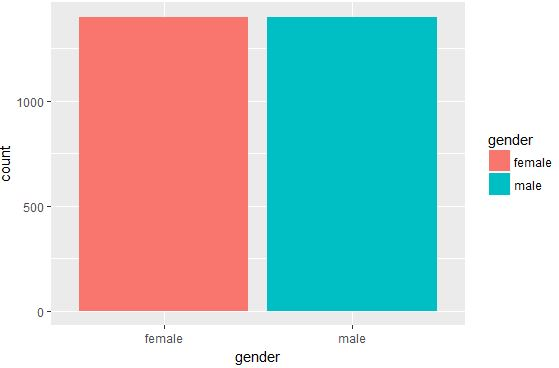
\includegraphics[width=0.5\textwidth]{GraficoGender}
\end{figure}

\begin{figure}
    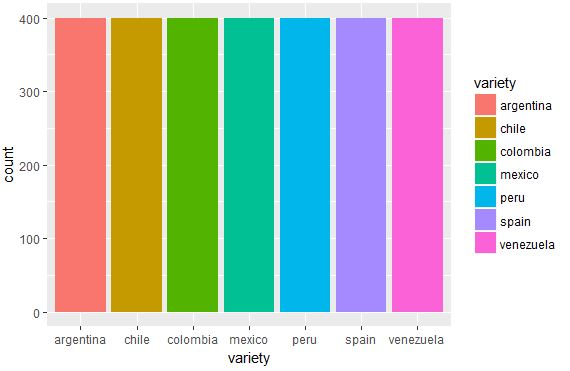
\includegraphics[width=0.5\textwidth]{variety}
\end{figure}

\section{Propuesta del alumno}
\justify
Para nuestra propuesta trabajaremos con modelos separados para clasificar por sexo y por idioma ya que se mejoran los resultados en lugar de si lo hici\'eramos de forma conjunta.\par\noindent
Seguimos con la estrategia de bolsa de palabras. Por cada una de las palabras calculamos su frecuencia de aparici\'on en el corpus. Nosotros creamos un vector con este resultado que denominamos diccionario. De estas palabras s\'olo nos quedamos con las 1000 primeras siendo el orden la frecuencia de aparici\'on, es decir, nos quedamos con las m\'as frecuentes.\par\noindent
No se tiene en cuenta la sem\'antica de las palabras ni su uso en el contexto, ya que una misma palabra dicha en el contexto de un hombre puede tener una connotaci\'on o significado diferente a lo dicho por una mujer. Esto queda fuera del estudio realizado. \par\noindent
La propuesta o hip\'otesis con la que mejor resultado obtuvimos fue en obtener una bolsa de palabras de mujeres, una bolsa de palabras de hombres y juntarlas en una \'unica. Al obtener las palabras exclusivas obtuvimos una mejora en el modelo. Este estudio lo hicimos para ambas clasificaciones de sexo y de idioma. \par\noindent
Sobre esta bolsa de palabras de la uni\'on de las exclusivas de cada sexo o variedad de idioma si añad\'iamos m\'as palabras con cierta exclusividad en cada clase mejoramos de nuevo el resultado. \par\noindent 
En la bolsa de palabras de la uni\'on de las exclusivas por clase añadimos algunas palabras. Estas fueron seleccionadas por la gu\'ia de estudios que afirman que las mujeres utilizan m\'as pronombres,negaciones, presente en tiempos verbales que los hombres, y que los hombres emplean m\'as adjetivos, determinantes y modificadores.  \par\noindent
Nos quedamos con una reducida bolsa, exactamente 417 palabras. Quer\'iamos complementar esta lista pero no seguimos con el estudio. \par\noindent

\section{Resultados experimentales}
\justify
Elegimos un modelo de regresi\'on lineal y de \'arboles pues tanto en la clasificaci\'on del sexo como del lenguaje nativo nos enfrentamos a clasificaci\'on por variable discreta. \par\noindent
La intuici\'on nos dice que separemos el vocabulario de las mujeres y de los hombres para la clasificaci\'on de sexo y lo mismo para las distintas clases de idioma. As\'i conseguir palabras significativas en la clasificaci\'on. \par\noindent
Realizamos varias hip\'otesis y fuimos anotando el resultado de accuracy. Pasamos a detallar estos resultados. \par\noindent
Las dos primeras hip\'otesis que nos planteamos fue pensar que si ten\'iamos una bolsa de palabras m\'as frecuentes para mujeres clasificar\'iamos mejor a las mujeres, y por tanto a los hombres. Lo mismo para el caso contrario.\par\noindent
\underline {Hip\'otesis 1}: Bolsa de palabras m\'as frecuentes para mujeres \par\noindent
Accuracy: 0,67 \par\noindent
\underline{Hip\'otesis 2}: Bolsa de palabras m\'as frecuentes para hombres \par\noindent
Accuracy: 0,68 \par\noindent
\underline{Hip\'otesis 3}: Bolsa formada por la uni\'on de las bolsas de palabras exclusivas de hombres y mujeres. Obtenemos una bolsa de 379 palabras. \par\noindent
Accuracy: 0,6957 \par\noindent
\underline{Hip\'otesis 4}: Bolsa formada en la hip\'otesis 3 m\'as la intersecci\'on de las bolsas de las hip\'otesis 1 y 2. \par\noindent
Accuracy: 0,6907 \par\noindent
\underline{Hip\'otesis 5}: Bolsa formada por la hip\'otesis 3 m\'as una lista reducida de palabras \par\noindent
Accuracy: 0,6979 \par\noindent
Para la clasificaci\'on de los autores de los tuits por su idioma se ha seguido las siguientes hip\'otesis.\par\noindent
\underline {Hip\'otesis 1}: Bolsa de palabras m\'as repetidas en cada pa\'is y exclusivas por pa\'is \par\noindent
Accuracy: 0,8393 \par\noindent
\underline {Hip\'otesis 2}: Utilizando la misma bolsa de palabras que en hip\'otesis 1 pero con clasificaci\'on randomForest de 50 \'arboles \par\noindent
Accuracy: 0,8507 \par\noindent
\underline {Hip\'otesis 3}: Bolsa de palabras con las 100 m\'as frecuentes de las exclusivas de cada pa\'is. \par\noindent
Accuracy: 0,7271 


\section{Conclusiones y trabajo futuro}
\justify
Las palabras utilizadas m\'as frecuentemente por una de las clases, ya sea sexo (hombre, mujer), o variedad en el idioma nativo (Colombia, Argentina, España, Venezuela, Peru, Chile, Mexico) cuando son comparadas con las otras clases son buenas caracter\'isticas para el modelo. \par\noindent
La cantidad de variables o caracter\'isticas tambi\'en es un punto muy importante para tener modelos eficientes y no solo en accuracy si no en tiempo o rendimiento, as\'i que, es primordial la selecci\'on de un buen n\'umero de variables. Adem\'as con nuestras hip\'otesis nos dimos cuenta que reduciendo el n\'umero de palabras de nuestro diccionario mejor\'abamos el resultado. \par\noindent
Por tanto, nuestro trabajo futuro ir\'ia encaminado a la selecci\'on de las palabras m\'as significativas para la clasificaci\'on en cada clase y en encontrar el n\'umero ideal de ellas para conseguir modelos eficientes. \par\noindent
Como modelos de clasificaci\'on utilizamos el de m\'aquinas de vector soporte y randomForest para el idioma. Quisimos probar con m\'as modelos pero tuvimos problemas con la herramienta RStudio y en futuros trabajos sabemos de la importancia de probar con distintos modelos y as\'i comparar resultados. 


\begin{thebibliography}{}
\bibitem[\protect\citename{Aho and Ullman}1972]{Aho:72}
Alfred~V. Aho and Jeffrey~D. Ullman.
\newblock 1972.
\newblock {\em The Theory of Parsing, Translation and Compiling}, volume~1.
\newblock Prentice-{Hall}, Englewood Cliffs, NJ.

\end{thebibliography}

\end{document}
